\documentclass[tikz,border=7pt]{standalone}
\usetikzlibrary{automata,positioning,arrows.meta}
\begin{document}
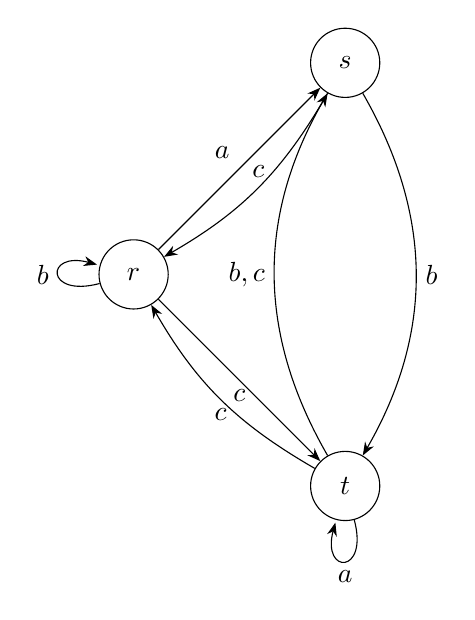
\begin{tikzpicture}[>=Stealth,node distance=3.8cm,on grid,auto]
\node[state] (r) {$r$}; \node[state] (s) [above right=of r] {$s$}; \node[state] (t) [below right=of r] {$t$};
\path[->] (r) edge[loop left] node {$b$} () edge node {$a$} (s) edge node[below] {$c$} (t)
 (s) edge[bend left] node {$b$} (t) edge[bend left=15] node[above] {$c$} (r)
 (t) edge[loop below] node {$a$} () edge[bend left] node {$b,c$} (s) edge[bend left=15] node[below] {$c$} (r);
\end{tikzpicture}
\end{document}
